\section{TinyDAS}

In this section, we introduce TinyDAS, a Python program aimed at training autoencoder models and detecting anomalies within \acrshort{das} data. 

\subsection{Tools}
\mycomment{
Python is a dynamically typed, weak language famously known for it's \textit{easy-to-learn} syntax. Created by Guido Van Rossum in the late 80-s \cite{python}, Python has slowly emerged as one of the fastest growing programming languages ever created \cite{srinath2017python}. 

Virtually all of the larger libraries for data science and \acrlong{ml} have bindings to \gls{python}, or are written in Python from scratch. Some examples include \texttt{Pandas}, \texttt{NumPy}, \texttt{SciKit Learn}, \texttt{Pytorch} and \texttt{TensorFlow}. Many of these rely on code written in C or C++ to be fast, sincc
}

In addition to \texttt{Tinygrad}, we will also be utilizing \texttt{Pytorch} for certain models, as \texttt{Float16} calculations appear to be a bit more stable for certain models. For anomaly detection, we utilize several popular Python packages such as \texttt{numpy}, \texttt{scikit-learn} and \texttt{seaborn} for evaluation metrics, and \texttt{matplotlib} for visualization and plots. A full list of packages used can be found in 
appendix \ref{app:tinypacks}.


\subsection{Overview}

TinyDAS consists of two parts. The first part handles model construction and training, while the latter deals with anomaly detection of \acrshort{das} data. An overview of how TinyDAS works is shown in figure \ref{fig:dataflow}. The following list outlines the fundamental philosophies and criteria used to design and evaluate the framework:

\begin{figure}[!h]
    \centering
    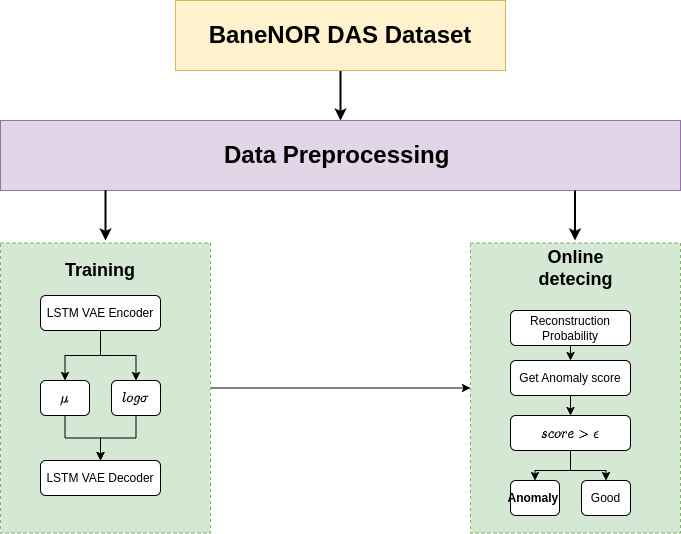
\includegraphics[scale=0.5]{figures/methodflow.png}
    \caption{Overview of TinyDAS}
    \label{fig:dataflow}
\end{figure}


\begin{enumerate}
    \item \textit{Support} for memory-efficient training techniques, specifically half-precision
    \item \textit{Scalability} from single-core systems to multi-node clusters
    \item \textit{Hardware agnostic} to ensure wide usability
    \item \textit{Modular architecture}, easily extendable with new models
    \item \textit{Separation of core logic} from data workflow for improved maintainability
    \item \textit{Collection} of different algorithms for anomaly detection
    \item \textit{Future potential} for online anomaly detection in a live environment
    \item \textit{Model-agnostic} approach to anomaly detection for broader applicability
\end{enumerate}

\subsection{Dataset}

For this project, we will be using datasets from the PubDAS \cite{spica2023pubdas} collection. PubDAS is described as "A PUBlic Distributed Acoustic Sensing Datasets Repository for Geosciences" and contains \acrshort{das} data from numerous location all across the globe. We will specifically be dealing with the FORESEE dataset, a \acrshort{das} dataset stored in \acrshort{hdf5} files from an area around Pennsylvania in the Valley and Ridge Appalachians region  as seen in \ref{fig:foresee}. \\

\begin{figure}[!h]
    \centering
    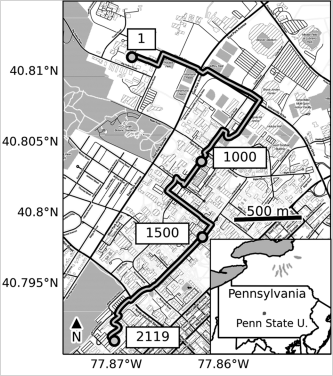
\includegraphics[width=0.5\linewidth]{figures/foresee.png}
    \caption{Map of the FORESEE Array. Photo is taken the PubDAS paper \cite{spica2023pubdas}}
    \label{fig:foresee}
\end{figure}

\begin{table}[!htbp]
    \centering
    \small
    \begin{tabular}{@{}p{0.3\textwidth}p{0.4\textwidth}p{0.2\textwidth}@{}}
        \toprule
        \textbf{Parameter} & \textbf{Value} & \textbf{Unit} \\
        \midrule
        Experiment & Foresee & \\
        Interrogator Unit (IU) & Silixa iDAS-v2 & \\
        Gauge length & 10 & \si{\meter} \\
        Cable length & 23300 & \si{\meter} \\
        Channel spacing & 2 & \si{\meter} \\
        \midrule
        \textbf{Original Data} & & \\
        Format & TDMS & \\
        Samples per second & 500 & \si{\hertz} \\
        File duration & 10 & \si{\minute} \\
        Data shape & 300000 \(\times\) 2137 & \\
        \midrule
        \textbf{After Preprocessing} & & \\
        Format & HDF5 & \\
        Samples per second & 125 & \si{\hertz} \\
        File duration & 5 & \si{\second} \\
        Data shape & 625 \(\times\) 2137 & \\
        \midrule
        \textbf{Dataset Information} & & \\
        Train dataset size & 25690 files & \\
        Train dataset span & 02 Mar 2020 08:10:15 to \newline 03 Mar 2020 20:40:10 & \\
        Labeled dataset size & 600 files & \\
        Labeled dataset span & 15 Apr 2019 03:17:35 to \newline 15 Apr 2019 04:07:30 & \\
        \bottomrule
    \end{tabular}
    \caption{FORESEE Experiment Data Summary}
    \label{tab:foresee_experiment_data}
\end{table}

PubDAS consist of 8 datasets stored in 3 different file formats. These 3 are \texttt{TDMS}, \texttt{HDF5} and \texttt{SEG-Y}. 
The FORESEE

\subsection{Data Preprocessing}

Some preprocessing on the dataset has already been done. This code is highlighted in the appendix \ref{app:pubdas}. To reduce the memory requirements of training such a dataset, we split the files into 5 second intervals compared to the original 10 minutes. Not only does this reduce memory requirements, but anomaly detection may be run every 5 seconds compared to the original 10 minutes. \\

Subsequentially, we chose a test dataset to label anomalies on based on this paper \cite{zhu2023seismic}, that found 18 thunder-induced seismic events in in this timestamp. We manually these data to be able to calculate confusion matrices and other relevant metrics to test the accuracy of our autoencoders. Information about these datasets can be found in table \ref{tab:foresee_experiment_data}. \\

When first downloading these data, they're stored in 10-minute files, resulting in quite large files as shown below:

\begin{align*}
\text{Size} &= 10 \times 60 \times 125 \times 2137 \times 4 \\
&= 600 \times 125 \times 2137 \times 4 \\
&= 641,100,000 \text{ bytes} \\
&\approx 641.1 \text{ MB} \\
&\approx 0.6411 \text{ GB}
\end{align*}

where:
\begin{itemize}
    \item 10 minutes is the duration of each file
    \item 60 seconds per minute
    \item 125\si{\hertz} is the sampling rate
    \item 2137 is the number of channels
    \item 4 bytes per sample (Float32)
\end{itemize}

Most consumer grade \acrshort{gpu}s can only store about 8-16gb of data in VRAM, thus meaning the batches of data we can store is not that big. Additionally, not only does the \acrshort{gpu}s have to store data, but also the weights and biases of the model, as well as losses and more. Motivated by this, we decide to split the files to last 5 seconds compared to 10 minutes. \\ 

We start of by looking at the file names and removing the prefix \textbf{FORESEE\_UTC\_}, since we're only working with one dataset at the time. Furthermore, in parallel fashion, we split each of the files in smaller ones, calculating new filenames based on the beginning timestamp. Now, each \acrshort{hdf5} file store a $625*2137$ matrix of \acrshort{das} data, successfully reducing the memory usage. 
These data are originally stored as \texttt{Float32}, but will be casted as \texttt{Float16} for faster training as we will see later on. In total, more than 25 000 files from the month of april 2020 is gathered to train our model on. 
RESULT: SPEAK ABOUT 5 SECONDS FOR LIVE ENVIRONMENT.
TODO: Inference data from 15042019!

\subsection{Models} 

We implementing four types of autoencoders: a linear autoencoder (AE), a convolutional autoencoder (CAE), a variational autoencoder (VAE), and a convolutional variational autoencoder (CVAE). The first model serves as a baseline to test against. In AE models, the latent space $Z$ can become disjoint and non-continuous, which VAE models try to solve. Additionally, we introduce convolutional layers in an attempt to improve the model's feature extraction capabilities. Based on this, these models serve as a baseline for what is to be expected by autoencoders for anomaly detection. A full list of layers and parameter sizes can be found in the appendix \ref{app:archs}. \\

\subsection{\acrshort{api} design}

Due to Tinygrad being a relatively simple framework, we implement components to be used for training and testing, with the intent of being reusable and modular.

\subsubsection{Datasets and Dataloaders}

The \texttt{Dataset} and \texttt{DataLoader} classes supports reading in \acrshort{hdf5} in batches, with support for data normalization and type casting. The former handles information about the dataset to be trained on, as well as logic for loading a single file from a \acrshort{hdf5} file, or whatever other format might be sent in later on. The latter one handles loading of batches in parallel, loading $n$ samples into the model.

\subsubsection{Autoencoder Base Class}

\lstinline{BaseAE} is the abstract class which all the different models inherit from. As long as all models inherits from this class, it will be run in the trainer. The \lstinline{criterion} method is the main method to call when training a model. It runs the \lstinline{__call__} method, applies the loss function of choice, and stores in a dictionary in case we'd like to save multiple losses across epochs. We define the class as follows:

\lstinputlisting[language=Python, label={lst:baseae}, caption=Base Autoencoder class]{code/baseae.py}

\subsubsection{Early Stopping}

Even though the model loss ideally should decrease to eventually reach zero almost immediately, this is never the case. Overfitting is when the loss starts increasing, never to return to its best value. To avoid spending time and resources on unnecessary training, we implement a useful mechanism called early stopping, which is described as follows:


\begin{align*}
&\text{Stop at epoch } T \text{ if:} \\
&\forall i \in \{T-p+1, ..., T\}: L_t(i) > L_t^* - \epsilon \\
&\text{where } L_t^* = \min_{j=1}^{T} L_t(j) \\
\\
&\text{Given:} \\
&L_t(t) \text{ is the train loss at epoch } t \\
&p \text{ is the patience (number of epochs to wait)} \\
&\epsilon \text{ is a small threshold for improvement}
\end{align*}

\subsubsection{Trainer}

The Trainer class serves as the core component of our program. As demonstrated in listing \ref{fig:lstmcell}, it integrates a model, dataloader, and optimizer to execute the training process. Additionally, it handles early stopping, storing history of losses and saving the best model for further use.

\lstinputlisting[language=Python]{code/trainer.py}


\subsubsection{Usage}

In the same way that \texttt{Judas} is designed, we want \texttt{TinyDAS} to be modular and easy to use. We've designed components in a way that is familiar to that of \texttt{Pytorch}. Models can be trained using the following script:

\lstinputlisting[caption=Example of how models within \texttt{TinyDAS} is trained, language=Python]{code/tinydas_main.py}

We allow for \texttt{Float16} training by type casting all weights and biases in the model, which effectively halves the memory requirement.

\subsubsection{Hyperparameters and configurations}

All hyperparameters for the different models are stored in separate YAML files. A list of hyperparameters used can be found in the appendix \ref{app:configs}.

\subsection{Evaluation}

We will be splitting the evaluation of the models in two sections. The first section will focus more on overall model training. Here is a list of points to be evaluated: 

\begin{itemize}
    \item \textbf{Experiment 1}: Median training time and model sizes, and losses
    \item \textbf{Experiment 2}: Reconstruction Capabilities
\end{itemize}

The second section will revolve around anomaly detection based on the different architectures. There are several different methods to evaluate the effectiveness and accuracy of models designed for anomaly detection. A very common pattern is to measure predicted results up against some ground truths, and construct a confusion matrix based on the result. From this confusion matrix, the following metrics will be used. \\ 

The True Positive Rate (TPR), also known as recall calculated the percentage of truths calcualted out of all ground truths. TP is true positives, and FN is false negatives. 

\begin{equation}
    TPR = \frac{TP}{TP + FN} = Recall
\end{equation}

Likewise, the False Positive Rate is the percentage of falsehoolds calculated out of all the ground negatives. FP is false negatives, and TN is true negatives:

\begin{equation}
    FPR = \frac{FP}{FP + TN}
\end{equation}

Precision is the percentage of correct truths out of all predicted truths.

\begin{equation}
    Precision = \frac{TP}{TP + FP}
\end{equation}


The $F1\_{score}$ is used to evaluate the balance between intrusion detection accuracy and recall rate; the higher the score, the better:
\begin{equation}
    F1\_{score} = 2 \times (\frac{Precision \cdot Recall}{Precision + Recall})
\end{equation}

Accuracy measures the proportion of correct predictions:

\begin{equation}
    Accuracy = \frac{TP + TN}{TP + TN + FP + FN}
\end{equation}


\begin{itemize}
    \item \textbf{Experiment 1}: Anomaly Detection Accuracy
    \item \textbf{Experiment 2}: Confusion Matrix and Metrics
\end{itemize}

